\chapter{Fundamentação Teórica}
\label{cap:estadoarte}

\section{Sistemas de Tempo Real}
Quando falamos de sistemas de tempo real \gls{str} logo pensarmos em sistemas de controle industrial ou em algum tipo de sistemas embarcado ultra rápido, porém os STR vão além destas aplicações, indo, em seus primórdios computacionais, da decodificação de mensagens inimigas aos modernos sistemas computacionais utilizados por instituições financeiras que por questões regulamentares precisam garantir que os tempos de suas transações estejam dentro do limite estipulado sem, no entanto, serem longas ao ponto de provocarem perdas monetárias. Essa vasta gama de aplicações nos mostra o quão heterogêneos são estes sistemas e o quanto diversificada são suas implementações, indo de sistemas implementados utilizando alguma linguagem de montagem em microcontroladores de 8 bits a supercomputadores que executam complexos sistemas operacionais sobre os quais aplicações ainda mais complexas são também executas.
 
Segundo \cite{Laplante2012},um sistema pode ser dito de tempo real quando sua correção lógica está relacionada tanto a correção das saídas produzidas pelo sistema quanto pela sua pontualidade, ou seja são sistemas que além de prezarem pela qualidade e correção dos seu algoritmos computacionais, também devem prezar pela pontualidade com que suas ações são tomadas, do contrario o sistema falhará.

Ao contrário do que diz o senso comum, um sistemas de tempo real não tem como principais objetivos a diminuição dos tempos de resposta a estímulos ou simplesmente ser extremamente veloz, um sistemas de tempo real tem como principal objetivo atender aos prazos estabelecidos no domínio do problema de forma determinística e por consequência previsível.
\cite{Farines2000} afirma que, um sistema de tempo real é previsível nos domínios lógico e temporal quando, independente das circunstâncias do hardware, carga ou falhas, pode-se saber com antecipação o seu comportamento antes da execução. A rigor, para que o comportamento do sistemas seja estabelecido de forma determinística é necessário conhecer todas as variáveis que compõem o ambiente em que o sistema está inserido como: hipóteses de falha, carga computacional, arquitetura do hardware, sistema operacional, linguagem de programação, etc, e que em cada fase do seu desenvolvimento metodologias e ferramentas sejam aplicadas na verificação do seu comportamento e previsibilidade.

\subsection{Classificação}
Existem diversas formas de se classificar os sistemas de tempo real, uma das formas mais comuns de faze-lo,  \cite{Farines2000} e \cite{Laplante2012}, é pela observação do rigor com que tratam seus requisitos temporais e no tipo de problemas que falhas relacionadas a esses requisitos podem provocar. Sendo assim, os sistemas, podem ser classificados como sendo do tipo \textit{soft} (brandos) ou \textit{hard} (rígidos). 

Um sistema de tempo real é brando quando o não cumprimento de suas restrições temporais provoca apenas alguma degradação no seu desempenho porém sem provocar falhas graves. Geralmente nesses sistemas os prejuízos provocados pela degradação do desempenho são compensados pelos benefícios de sua operação normal.

Um sistema de tempo real é rígido quando a falta no cumprimento de uma única restrição temporal pode levar a uma falha catastrófica. Nesse caso, uma falha no cumprimento de um prazo provoca prejuízos infinitamente maiores, como: uma catástrofe ambiental, a perda de vidas humanas ou grandes perdas materiais, que as benesses do sistema em operação normal.

\cite{Laplante2012} ainda estabelece uma terceira classificação entre os sistemas brandos e rígidos, o sistema de tempo real firme, onde se enquadram sistemas em que a perda de uma quantidade limitada de prazos não compromete o desempenho de forma crítica, porém a extrapolação do limite de prazos perdidos leva a uma falha catastrófica.

\subsection{Tarefas de Tempo Real}
Como todo sistema computacional, STR executam uma ou um conjunto de tarefas com o objetivo de produzir algum trabalho útil. \cite{Kopetz2002} as define simplesmente como a execução de um programa sequencial, iniciando-se, normalmente, com a leitura de alguns dados de entrada e findando com a produção de algum resultado e alterando seu estado interno. 

Uma tarefa pode se classificada como de tempo real se obedece aos dois preceitos básicos definidos anteriormente para sistemas de tempo real, os seja sua correção lógica está ligada a correção de suas saídas e a correção temporal, estando sujeitas ao cumprimento de prazos (\textit{deadline}), e assim como os sistemas de tempo real, uma tarefa é dita crítica ou rígida, quando o não cumprimento de seus prazos pode provocar alguma falha catastrófica, e branda quando não lhes cumprir provocam, no máximo, uma diminuição do desempenho, sem grandes consequências.

As tarefas de tempo real, também são classificadas quanto a regularidade de sua ativação podendo ser periódicas, quando sua ativação ocorre em intervalos regulares predefinidos, ou como aperiódicas quando sua ativação ocorre de modo aleatório, normalmente em resposta a algum evento externo ou interno ao sistema. Quando executam múltiplas tarefas os sinais que determinam o inicio (ativação) e termino de uma tarefa são controlados pelo escalonador do sistema.

Quando um sistema executa múltiplas tarefas é necessária a implementação de um algoritmo de escalonamento. O escalonador é definido por \cite{Farines2000} como o componente do sistema que é responsável pela implementação das políticas de acesso e gerenciamento de uso do processador pelas tarefas. Quando o número de tarefas em execução simultânea é maior que o número de unidades de processamento disponíveis no sistema, além de um escalonador, o sistema deve prover algum mecanismo capaz de guardar o estado atual do processador associado as tarefas para que posteriormente esse estado possa ser carregado novamente e a execução retomada do ponto onde parou, este processo é chamado de chaveamento de contexto. Dentro deste cenário, segundo \cite{Tanenbaum2009}, uma tarefa pode assumir diversos estados conforme a figura \ref{EstadoProcesso}.

\begin{figure}[!htb]
    \centering
    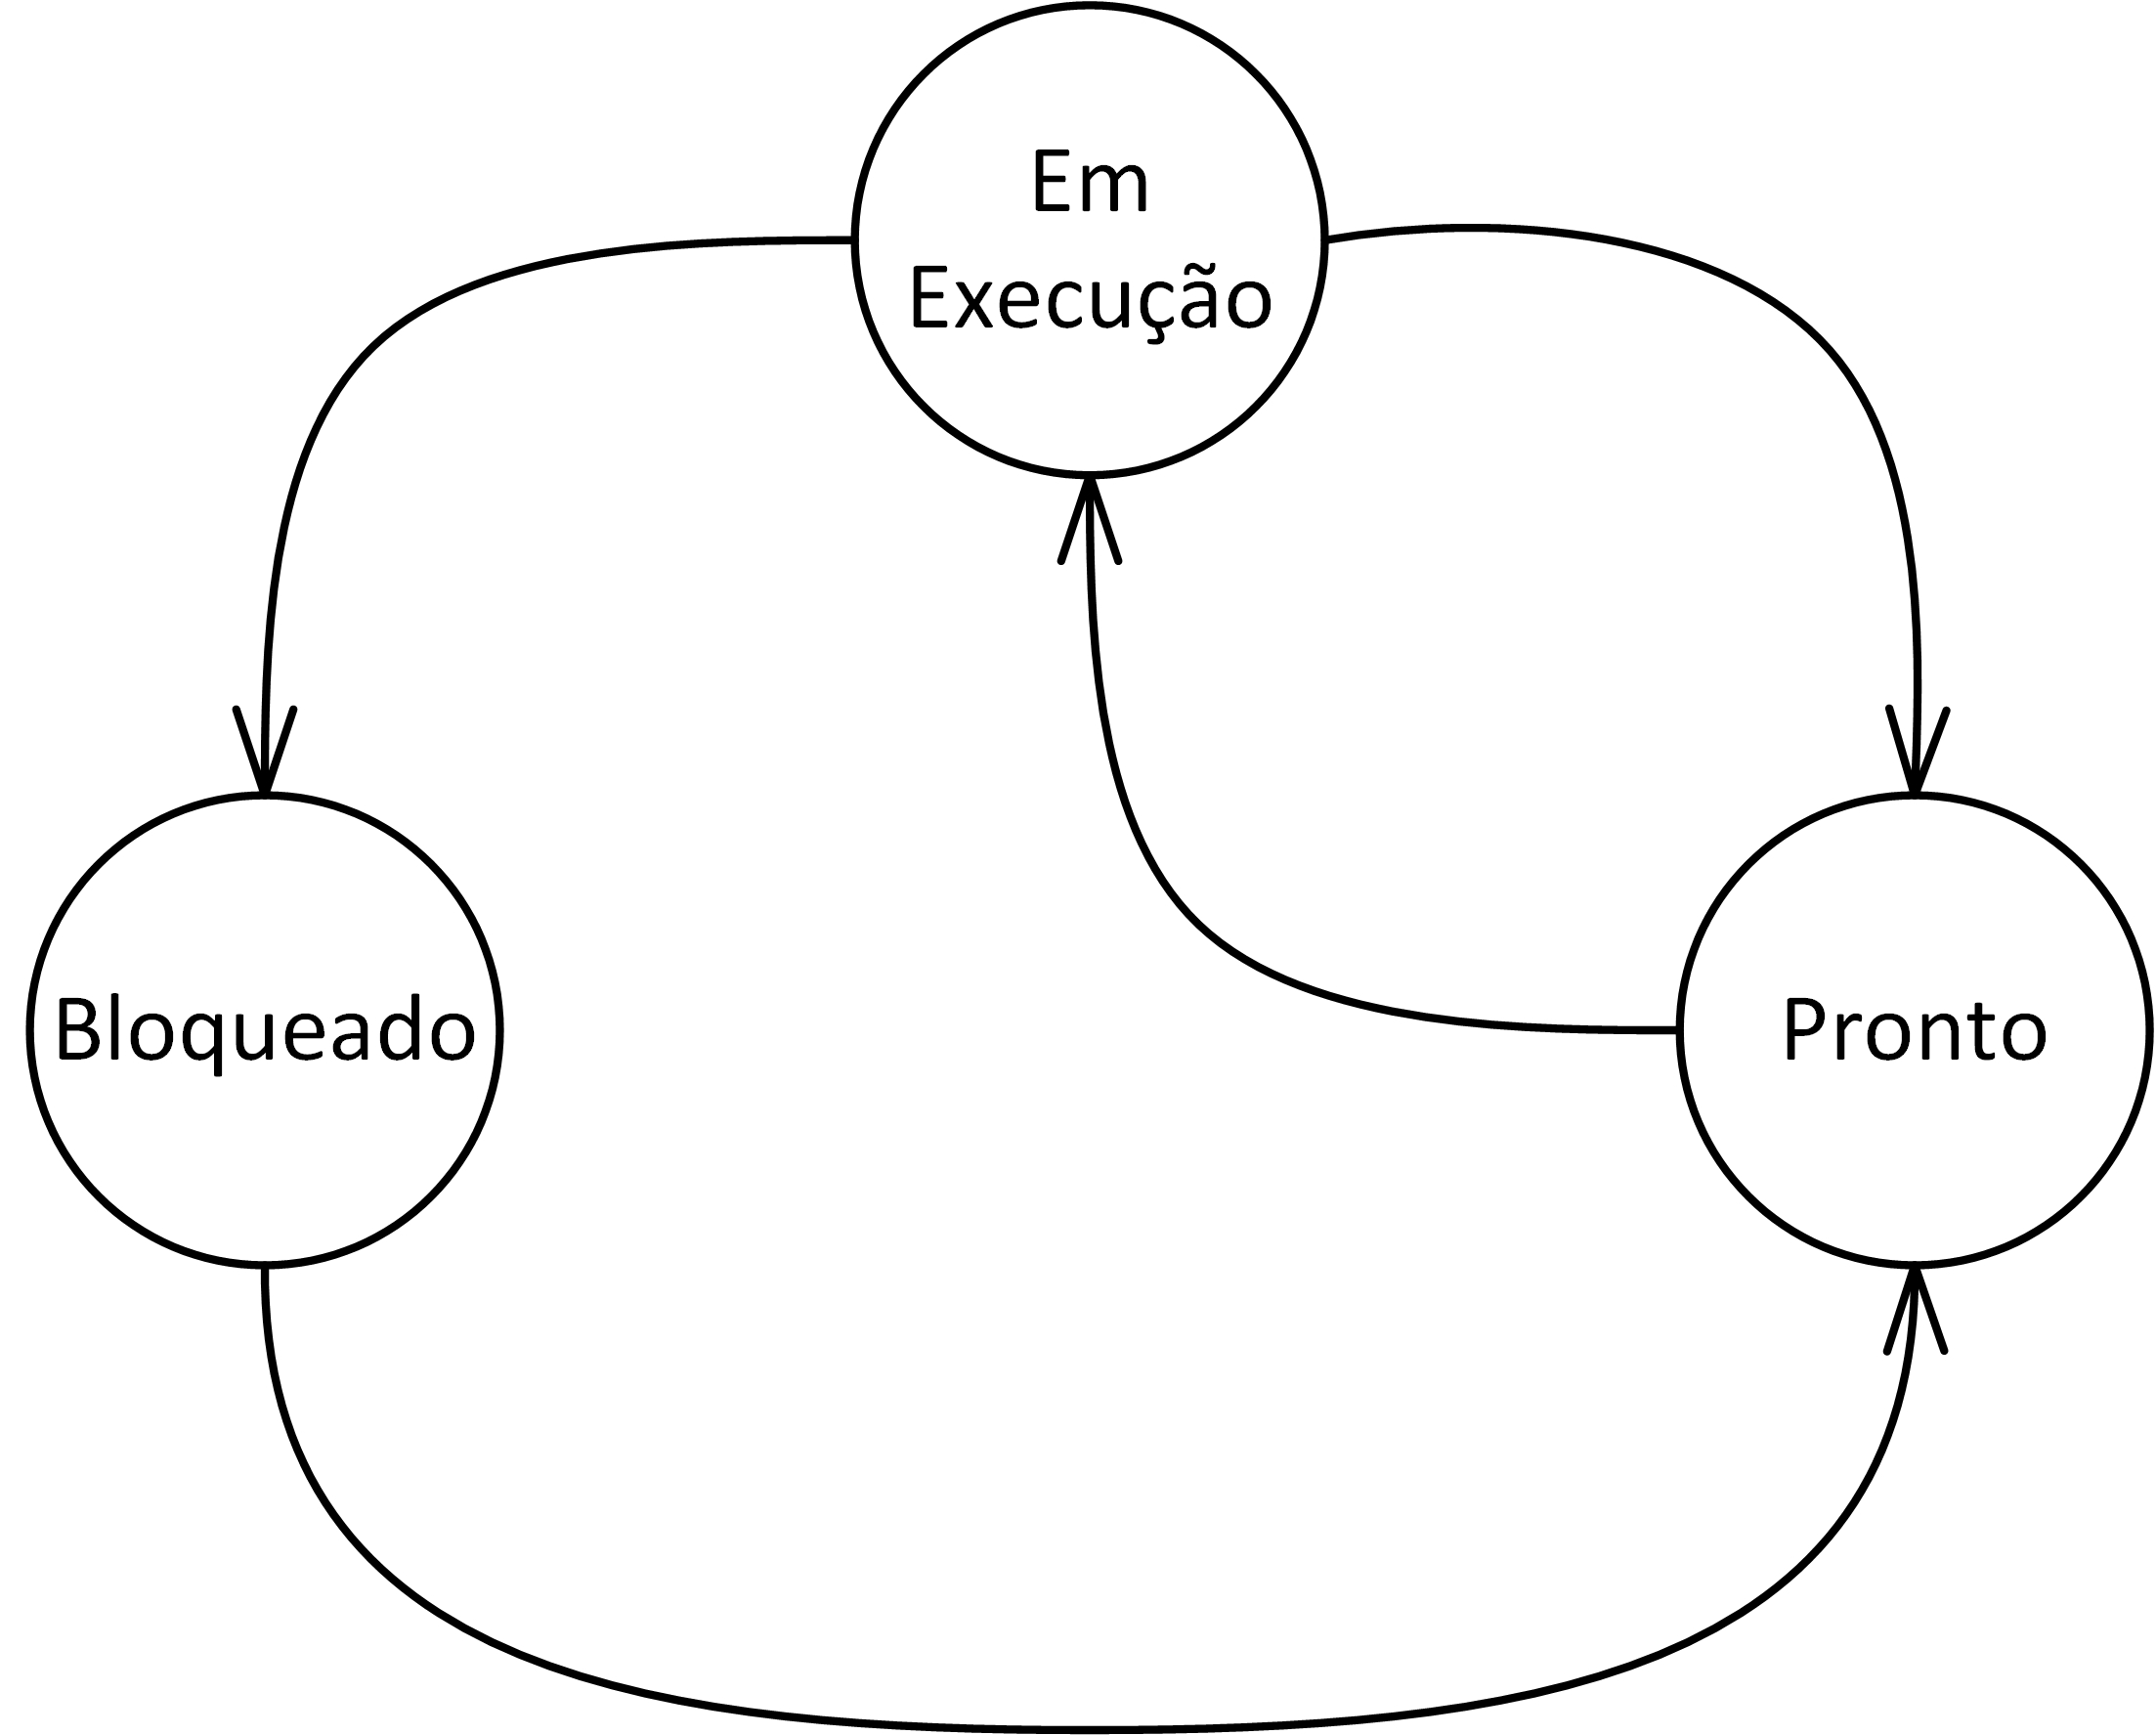
\includegraphics[scale=0.6]{EstadosProcesso}
    \caption{Estados de uma tarefa e seus relacionamentos}
    \label{EstadoProcesso}
\end{figure}

Na modelagem de tarefas de tempo real são utilizados alguns parâmetros que definem seu comportamento temporal: tempo de computação (Tc), tempo inicial (Ti), tempo final (Tf), tempo de liberação (Tl), \textit{deadline} (D) e, caso a tarefa em questão seja periódica, o período (P). O tempo de computação corresponde ao tempo total exigido para que a tarefa seja completada. Os tempos inicial e final correspondem aos instantes em que a tarefa inicia e finaliza, respectivamente, sua execução durante uma janela de ativação. O tempo de liberação é o momento em que uma tarefa entra no estado de "Pronto". O \textit{deadline}, como já foi dito, é o prazo máximo que uma tarefa tem para concluir sua execução. E o período corresponde ao intervalo de tempo com que a tarefa repete sua execução. Outro parâmetro que deve ser considerado, principalmente quando trabalhamos com múltiplas tarefas e que é usado por diversos algoritmos de escalonamento, é a prioridade(PR, que representa a urgência relativa de execução de uma tarefa em relação as outras. O conhecimento desses parâmetros é bastante importante para garantir a previsibilidade do sistema, além de possibilitarem a verificação da viabilidade, montar as tabelas e definir as políticas, de escalonamento. Os parâmetros de tempo estão ilustrados na figura \ref{TemposTarefa}.
 
\begin{figure}[!htb]
    \centering
    \includegraphics[scale=0.7]{TemposTarefa}
    \caption{Características temporais de uma tarefa de tempo real}
    \label{TemposTarefa}
\end{figure}

\section{Sistemas Operacionais de Tempo Real}
Com o aumento da complexidade das aplicações de tempo real \gls{atr} e consequentemente do hardware utilizado na execução das aplicações de tempo real, ouve também um aumento na complexidade do trabalho realizado pelos desenvolvedores de aplicações. Para contornar parte desse problema a utilização de sistemas operacionais de tempo real \gls{sotr} tornou-se cada vez mais comum. outro ponto importante, é o fato de que é bastante comum ATR possuírem  algumas funcionalidades que não possuem restrições temporais como interações com banco de dados, acesso a internet, interfaces gráficas, etc, e que sem o uso de um sistema operacional, implementar estes recursos é um processo bastante exaustivo.  

Segundo \cite{Tanenbaum2009}, um sistema operacional \gls{so} é um dispositivo de software que tem como principal finalidade fornecer um ambiente em que certas funcionalidades do sistema possam ser gerenciadas de forma autônoma e oculta ao desenvolvedor, proporcionando uma camada de abstração com um conjunto próprio de instruções sobre a qual o desenvolvedor possa maximizar seu trabalho utilizando uma interface de programação mais amigável.

Estendendo essa definição aos STR podemos dizer que um SOTR, além de possuir os principais objetivos comuns aos SO, deve criar um ambiente de desenvolvimento previsível e determinístico qualquer que seja a carga do sistema. Um SOTR deve fornecer um ambiente no qual ATR tenham seus requisitos temporais respeitados e executar de modo que suas ações possam ser previstas. Como geralmente são sistemas reativos, SOTR devem atender a requisitos relacionados a responsividade. Um SOTR deve garantir que respostas a estímulos, sejam internos ou externos, sempre serão dadas dentro de um intervalo de tempo que respeite os requisitos do sistema.

Assim como dito para os STR, um SOTR não tem como principais objetivos a redução dos tempos de resposta a estímulos ou ter uma performance superior quando comparado a um Sistemas Operacionais de Proposito Geral \gls{sopg}. SOTR de qualidade podem ter desempenho global semelhante a SOPG, porém o primeiro, normalmente, sacrificará a performance em detrimento da previsibilidade. SOPG podem, em 99,9\% dos casos, executar tarefas num tempo menor que SOTR, todavia nos 0,1\% dos casos restantes, o tempo de execução de uma tarefa será imprevisível, podendo ser até 1000 vezes mais longo que em um SOTR, isso seria mais que suficiente para reprovar o sistema em uma aplicação crítica. Embora a execução de tarefas em um SOTR possam ser executadas num tempo maior, são executadas com a garantia de estarem sempre dentro dos  prazos estabelecidos.

Dentre as principais funções de um SOTR, está o fornecimento mecanismos e ferramentas para que seja possível a execução de ATR de modo previsível e satisfatório aos requisitos impostos pelo domínio do problema. Os mecanismos oferecidos devem possibilitar ao desenvolvedor avaliar se o SOTR em questão é adequado ou não para a execução das aplicações pretendidas, isso inclui tornar acessível conhecer os valores de tempo máximo de execução de suas chamadas de sistema, os valores máximos das latências provocadas pelas operações internas do sistema e os valores de tempo relacionados as ATR. É importante observar que a qualidade dos valores apresentados está diretamente ligada a granularidade dos temporizadores disponibilizados pelo sistema, quanto maior for a resolução dos temporizadores melhor a qualidade das medições. Estes valores de tempo também podem variar de acordo com a arquitetura do processador em que o sistema é executado, com o código gerado pelo compilador utilizado para produzir o sistema, com os algoritmos utilizados nos processos internos do sistema e com a qualidade das suas respectivas implementações.

Alguns SOTR, como o FREERTOS descrito em \cite{Barry2016}, fornecem ao desenvolvedor apenas um conjunto mínimo de funcionalidades: suporte a multitarefa, escalonador com diversas políticas de escalonamento, \textit{mutex}, semáforos e temporizadores. Estes pequenos SOTR, também chamados de núcleos de tempo real ou \textit{ real time kernel}, são pensados para serem pequenos, velozes e capazes de implementar políticas de tempo bastante rígidas. Suas características se aplicam muito bem a sistemas embarcados baseados em microcontroladores e que trabalham com restrições temporais bastante rígidas.

Os grandes sistemas operacionais como: Linux, Windows Mac OS X, oferecem outros recursos mais avançados: serviços de entrada e saída de dados, proteção de memória, sistemas de arquivos, políticas de segurança, interface com o usuário etc. Estes recursos tornam possível ao desenvolvedor construir e executar aplicações mais complexas que proporcionam um maior nível de segurança e interação com outros sistemas e usuários. Nativamente estes sistemas não foram projetados para atender aos requisitos dos STR, porém seus desenvolvedores vem desenvolvendo alternativas para este fim como as diferentes versões do Windows Embedded e os \textit{patchs} disponibilizados para Linux: Preempt\_RT e RTAI. Vale lembrar que muitos dos sistemas em que se baseiam alguns SOTR, como Linux, já são utilizados em várias aplicações de missão crítica, além de que sistemas de controle baseados em PC são uma realidade na indústria como complemento e até substitutos aos tradicionais CLPs como os (\textit{Siemens PC-based Automation}). Estes sistemas permitem uma maior flexibilidade na programação, expansão e configuração de software e hardware.

\subsection{Latência}
Segundo o dicionário \cite{Priberam}, latência é o tempo decorrido entre o estímulo e a resposta correspondente.

No caso de sistemas computacionais e mais especificamente em SO, um estímulo, pode ser externo, que necessita de uma resposta do sistema, ou interno, como uma \textit{thread} que foi colocada no estado "pronto" e espera para ser executada.

Assim como todos os sistemas reais, SOTR, estão sujeitos a latências que surgem como consequência do seu próprio funcionamento e do hardware sobre os quais executam. O conhecimento dos valores de latência e principalmente sua constância, mesmo que em um cenário de sobrecarga do sistema, são primordiais na garantia da previsibilidade. O conhecimento dos valores de latência também são de vital importância na seleção de um SOTR que seja capaz de atender aos requisitos temporais de uma aplicação. Conforme \cite{Rostedt2007}, são causas comuns de latência em SO: latência de interrupção, latência de escalonamento, latência por inversão de prioridade, latência por inversão de interrupção.

A latência de interrupção corresponde ao tempo decorrido entre a ocorrência de uma interrupção e o momento em que é atendida. Há também o tempo entre o atendimento da interrupção e a rotina que realmente processará o sinal recebido. O tempo decorrido entre o despertar de um processo de alta prioridade e a sua execução as vezes podem ser consideradas latência de interrupção, uma vez que o seu despertar muitas vezes ocorre devido a algum evento externo. 

A latência provocada pelo escalonamento, é o tempo entre o instante em que uma tarefa de alta prioridade acorda ( tempo de liberação) e o momento em que ela inicia a execução (tempo inicial). 

As latências por inversão de prioridade e inversão de interrupção consistem no tempo que uma \textit{thread} com prioridade alta espera para utilizar algum recurso em uso por uma \textit{thread} de prioridade baixa, seja ela associada a uma outra tarefa ou, no caso da interrupção, a um manipulador de interrupções. Diferente da inversão de prioridade e inversão de interrupção não pode ser antecipada visto que a ocorrência da maior parte das interrupções não pode ser prevista.

\subsection{Linux Para Tempo Real}
As modernas aplicações de tempo real estão muito mais conectadas e iterativas, isso exige a implementação de novas funcionalidades, como interfaces gráficas, comunicação com serviços web e banco de dados. Essas funcionalidades além de um grande reuso de código, também fazem necessário um melhor suporte dos sistemas operacionais sobre as quais executam. Os SOTR tradicionais e os núcleos de tempo real, embora tenham um ótimo desempenho no cumprimento de metas temporais, geralmente, oferecem pouco ou nenhum suporte aos recursos utilizados nas aplicações mais modernas.

Na busca por melhor suporte as aplicações, vários projetos tomaram a iniciativa de incorporar funcionalidades de tempo real a SOPG. Devido ao seu código fonte aberto, sua comprovada robustez em aplicações críticas e sua portabilidade entre diferentes plataformas de hardware, o Linux, tornou-se um dos sistemas mais utilizados nas conversões para tempo real. Porém o Linux é concebido para uso e computadores pessoais e servidores e por este motivo seu \textit{kernel} é otimizado para obter um melhor desempenho global e alocar recursos de forma justa para todos os processos em execução por meio do seu escalonador Completely Fair Agendador \cite{cfs}. 

Dentre os projetos mais ativos, no trabalho de transformar o Linux em um SOTR, podemos citar: RTAI, Xenomai e Preempt\_RT. Cada um desses projetos implementa uma versão modificada do \textit{kernel}, com arquitetura própria, vantagens e desvantagens. Neste trabalho as soluções estudadas e avaliadas são o RTAI e o \textit{patch} Preempt\_RT.

\subsection{O \textit{Patch} PREEMPT\_RT}
O \textit{patch} Preempt\_RT é a solução de tempo real oficialmente suportada pelo \textit{kernel} Linux. Este projeto é a solução mais bem sucedida no esforço para transformar o Linux em um SOTR sem o auxilio de um \textit{microkernel}.

As modificações impostas pelo \textit{patch} Preempt\_RT ao \textit{kernel} incluem, a transformação de alguns manipuladores de interrupção em \textit{threads} de baixa prioridade (manipuladores de interrupção importantes para o funcionamento do sistema como um todo, como o temporizador, são mantidas com prioridade máxima), substituição das \textit{spin\_locks} por \textit{mutexes} para permitir que as regiões críticas do \textit{kernel} passem a ser preemptíveis, herança de prioridade. Algumas alterações não são mais necessárias pois foram incorporadas ao ramo principal do \textit{kernel}, como temporizadores de alta resolução e \textit{mutexes} no espaço de usuário.

As funcionalidades do sistema de forma geral permanece a mesma para gerenciamento, comunicação e sincronia entre \textit{threads}, com exceção de três novos modos de escalonamento, \textit{First In First Out} (FIFO) orientado a prioridades (em que 99 é a prioridade máxima), \textit{Round Robin} (RR), e \textit{Earliest Deadline First} (EDF).

\subsection{O RTAI}
O RTAI, acrônimo de \textit{Real-time Application Interface}, surgiu como uma variação do antigo \textit{RTLinux} desenvolvida pelo \textit{Dipartimento di Ingeneria Aerospaziale} da Universidade \textit{Politecnico di Milano}.

Sua abordagem para a transformação do Linux em um SOTR utiliza um \textit{microkernel} em paralelo ao \textit{kernel} do Linux que é responsável pela execução das tarefas de tempo real, enquanto o \textit{kernel} fica responsável pela execução das tarefas de baixa prioridade, está solução é comumente chamada de \textit{Dual Kernel}. Neste sistema o gerenciamento do hardware fica a cargo de uma camada de abstração criada abaixo dos \textit{kernels}, chamada \textit{ADEOS} (\textit{Adaptive Domain Environment for Operating Systems}). Esta camada é quem permite dois  núcleos compartilhare o mesmo hardware simultaneamente. A arquitetura implementada pelo sistema é ilustrada na figura.

\begin{figure}[!htb]
    \centering
    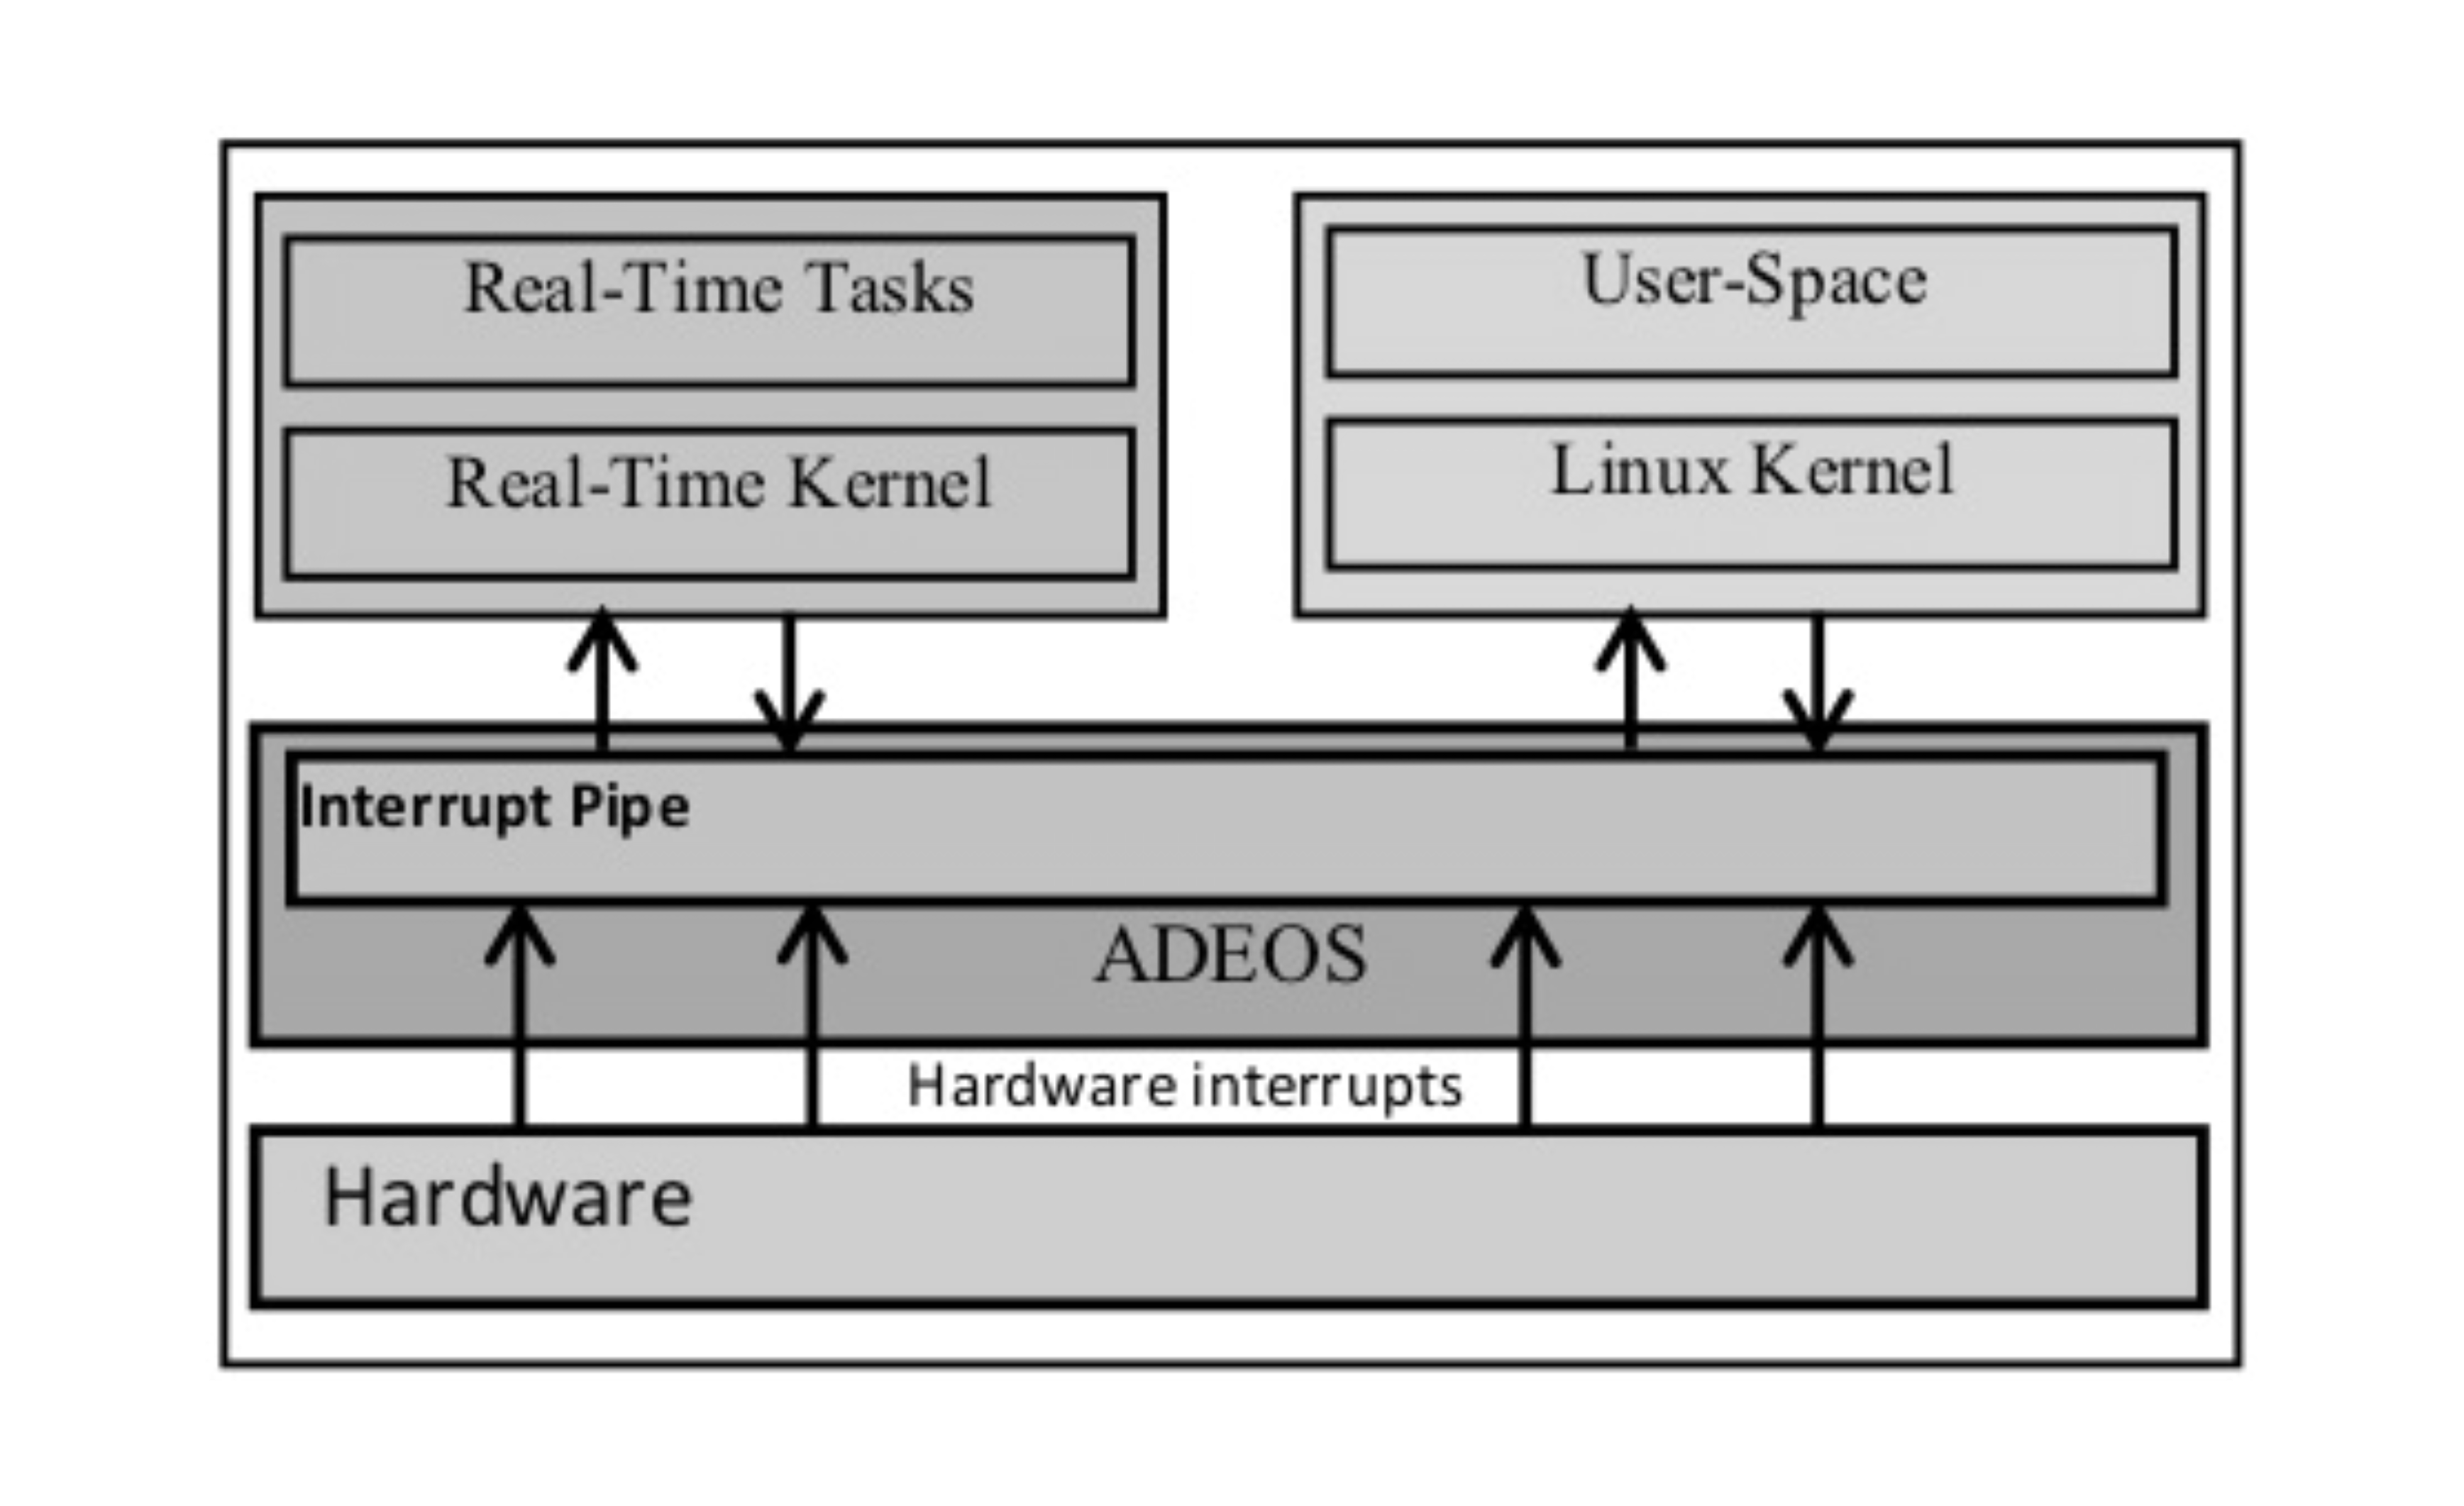
\includegraphics[scale=0.8]{ArquiteturaRTAI}
    \caption{Arquitetura \textit{Dual Kernel} adotada pelo RTAI, \cite{Litayem2011}}
    \label{TemposTarefa}
\end{figure}

O \textit{microkernel} implementado pelo RTAI, a semelhança dos NTR, suporta todo o conjunto básico de funcionalidades para a construção de ATR, como rotinas para a criação, destruição, suspensão, sincronia e comunicação entre tarefas, temporizadores com alta resolução, políticas de escalonamento, capacidade de execução de tarefas de tempo real no espaço do usuário e mecanismos para controle de recursos compartilhados. Seu escalonador suporta políticas \textit{Rate Monotonic} (RM), EDF, FIFO orientado a prioridades ( em que 0 é a maior prioridade) e RR.

